% ============================================================================
% GFD: Nuclear binding energy from the bidirectional scalar-tensor transition
% Figures: gfd_binding_two_curves, gfd_sierpinski_packing_8, gfd_shell_decomposition_4
% ============================================================================
\documentclass[fleqn,usenatbib]{mnras}

\usepackage{amsmath,amssymb}
\usepackage{graphicx}
\hypersetup{hidelinks}

\title{Nuclear Binding Energy from the Bidirectional Scalar-Tensor Transition}

\author[S. Nelson]{Stephen Nelson$^{1}$\thanks{E-mail: stephen@fielddynamics.org}\\
$^{1}$Field Dynamics Research}

\date{March 2026}
\pubyear{2026}

\begin{document}

\maketitle

% ----------------------------------------------------------------------------
% ABSTRACT
% ----------------------------------------------------------------------------
\begin{abstract}
The nuclear binding energy curve and the nuclear magic numbers are among the most precisely measured quantities in physics. The standard treatment fits the curve with five adjusted parameters and explains the magic numbers by introducing a phenomenological spin-orbit coupling term. We show that the scalar-tensor transition (SST), the same field equation used to decode galaxy rotation curves, has a quadratic partition that reproduces both results with zero free parameters. The SST quadratic, evaluated at each position of a 64-step walk set by the structural constants $K\!=\!4$ and $D\!=\!3$, yields (i) the seven nuclear magic numbers 2, 8, 20, 28, 50, 82, 126 from a closed-form packing formula, including the anomalous $20\!\to\!28$ gap without spin-orbit coupling; (ii) the binding energy per nucleon from helium to lead at a mean absolute error of 95\,keV; and (iii) a visual packing structure that connects the shell closures to the energy curve. All three results are independently reproducible from the equations presented here.
\end{abstract}

\begin{keywords}
nuclear structure -- nuclear binding energy -- magic numbers -- scalar-tensor theory -- gravitation
\end{keywords}

% ----------------------------------------------------------------------------
% 1. INTRODUCTION
% ----------------------------------------------------------------------------
\section{Introduction}
\label{sec:intro}

Every atomic nucleus is a balance sheet. Protons and neutrons bind together, and the energy cost of pulling them apart, the binding energy per nucleon $B/A$, follows a curve that rises steeply from hydrogen, peaks near iron, and gently declines through the heavy elements to lead. This curve is one of the most precisely measured quantities in all of physics, known to fractions of a kiloelectronvolt for hundreds of isotopes.

The standard description of this curve is the Bethe-Weizs\"acker semi-empirical mass formula, introduced in the 1930s. It fits the data well, but it requires five adjusted coefficients: volume, surface, Coulomb, asymmetry, and pairing, each calibrated to the data it is meant to describe. The formula is descriptive, not derived: it tells us \emph{what} the binding energy is, but not \emph{why} it takes the values it does.

A second challenge accompanies the curve. Nuclei with certain ``magic'' numbers of protons or neutrons, specifically 2, 8, 20, 28, 50, 82, and 126, are exceptionally stable. The first three follow naturally from a simple shell model, but the sequence $20\!\to\!28$ does not: the expected shell capacity at that level is far larger than 8. In 1949, Mayer and Jensen showed that adding a spin-orbit coupling term to the nuclear potential reproduces the correct sequence \citep{Mayer1949}. The correction is effective, but phenomenological: its strength and form are adjusted to match the observed magic numbers, rather than derived from a deeper principle.

This letter presents a single equation that addresses both problems. The equation is the quadratic partition of the scalar-tensor transition (SST), the same field equation that relates source to observed acceleration in galaxy rotation curves. When evaluated at each position of a structured walk with 64 steps, it reproduces the magic numbers from a closed-form packing formula and the binding energy curve from helium to lead at 95\,keV mean absolute error, with no free parameters. The $20\!\to\!28$ gap emerges from the structure itself, without spin-orbit coupling.

% ----------------------------------------------------------------------------
% 2. FRAMEWORK
% ----------------------------------------------------------------------------
\section{Framework}
\label{sec:framework}

\subsection{The scalar-tensor transition}
\label{sec:sst}

The covariant framework rests on a single action:
\begin{equation}
S = \int d^4 x\,\sqrt{-g}\,\bigg[ \frac{R}{16\pi G} - \frac{a_0^2}{8\pi G}\,F(y) - \frac{1}{4}\,e^{-2\Phi/c^2}F_{\mu\nu}F^{\mu\nu} + \mathcal{L}_{\mathrm{matter}} \bigg]
\label{eq:action}
\end{equation}
where $y = |\nabla\Phi|^2/a_0^2$. In the spherically symmetric limit, the scalar sector yields the scalar-tensor transition (SST):
\begin{equation}
g_{\mathrm{s}} = \frac{g_{\mathrm{t}}^2}{a_0 + g_{\mathrm{t}}}
\label{eq:sst}
\end{equation}
which relates the source acceleration $g_{\mathrm{s}}$ (from the mass distribution) to the total acceleration $g_{\mathrm{t}}$ (governing orbits). The constitutive law that follows from Eq.~\ref{eq:sst} is
\begin{equation}
\mu(x) = \frac{x}{1+x}
\label{eq:mu}
\end{equation}
where $x = g_{\mathrm{t}}/a_0$. This function describes what fraction of the field's total coupling capacity is active at a given acceleration.

In a previous letter \citep{Nelson2026}, we showed that Eq.~\ref{eq:sst}, combined with the Poisson equation and the constants $G$ and $a_0$, decodes effective mass from observed galaxy rotation curves with no free parameters. In that application, matter sources the field and the field governs orbits. The SST operates in one direction at a time.

\subsection{The SST quadratic: the bound-state partition}
\label{sec:quadratic}

In a nucleus, the situation is different in one important respect. Nucleon A binds to nucleon B, and nucleon B binds to nucleon A. Both are simultaneously source and response. The SST must be consistent in both directions at once.

Consider a pair of nucleons coupled through the SST. Let $\mu$ be the fraction of the coupling capacity used in one direction, so that the remaining capacity available for the return coupling is $(1 - \mu)$. In the one-directional case (Eq.~\ref{eq:mu}), $\mu = x/(1+x)$ and the return direction is unconstrained. In a bound state, self-consistency requires that the return coupling $(1 - \mu)$, acting as the effective source through the SST, produces exactly $\mu$ as its output. Substituting $(1-\mu)$ for the coupling fraction in the SST relation gives
\begin{equation}
x\,(1 - \mu)^2 = \mu
\label{eq:selfconsistent}
\end{equation}
which is a quadratic in $\mu$. The physical solution (the root that satisfies $0 < \mu < 1$ for $x > 0$) is
\begin{equation}
\mu_{\mathrm{SST}}(x) = \frac{(2x+1) - \sqrt{4x+1}}{2x}.
\label{eq:musst}
\end{equation}
This is the SST quadratic: what the scalar-tensor transition becomes when the field must close on itself in a bound state.

\subsection{Structural constants}
\label{sec:constants}

Two structural constants set the geometry of the walk. They come from a single uniqueness condition: the requirement that the number of linear degrees of freedom in the structure, $2(D+1)$, equals the number of states it can encode, $2^D$:
\begin{equation}
2(D+1) = 2^D.
\label{eq:uniqueness}
\end{equation}
The only integer solution is $D = 3$, which gives $K = D + 1 = 4$. Here $K$ is the branching factor (each level of the structure splits into four) and $D$ is the depth (three levels of subdivision). The walk through this structure has $K^D = 4^3 = 64$ positions.

These two integers are the unique values for which the field structure closes. Everything that follows, the walk length, the gate threshold, the magic numbers, the energy scale, uses only $K\!=\!4$ and $D\!=\!3$.

\subsection{The walk}
\label{sec:walk}

The structure defined by $K$ and $D$ is a Sierpi\'nski triangle: an equilateral triangle subdivided $D = 3$ times at branching factor $K = 4$, producing $K^D = 64$ sub-triangles. Each sub-triangle is one position in the walk.

The walk has four faces at the top level (indexed 0--3). Each face contains four channels, and each channel contains four sub-channels, giving $4 \times 4 \times 4 = 64$ positions. These 64 positions constitute one sector of the parent Sierpi\'nski triangle, which itself has $K = 4$ sectors for a total capacity of $4 \times 64 = 256$ positions. The fourth face at each level (index 3) is the \emph{gate face}: the boundary where the walk cycles back on itself. This distinction between ordinary faces and the gate face will determine both where shells close and where the binding curve reflects (Sec.~\ref{sec:faces}).

Nucleons fill the walk sequentially, from position 1 to position $A$. Each filled position contributes coupling $\mu_{\mathrm{SST}}(i^2)$ to the collective binding, where $i$ is the walk position and $x = i^2$ maps position to acceleration ratio. The squared mapping arises because the walk compresses spatial positions into the acceleration variable of the SST: the Jacobian of the transformation from position space to acceleration space is $dx = 2i\,di$, so $x = i^2$ is the natural coordinate.

% ----------------------------------------------------------------------------
% 3. RESULTS
% ----------------------------------------------------------------------------
\section{Results}
\label{sec:results}

The SST quadratic yields three results: the magic numbers (discrete and algebraically exact), the binding energy curve (quantitative and fully reproducible), and the Sierpi\'nski walk that connects them visually.

\subsection{Magic numbers from packing algebra}
\label{sec:magic}

The walk described in Sec.~\ref{sec:walk} has an internal shell structure set by $K$ and $D$. Nucleons fill the walk sequentially, and the positions pack into concentric layers indexed by $n = 1, 2, 3, \ldots$\,. The shells close at cumulative counts given by a packing formula. Define the tetrahedral number
\begin{equation}
T(n) = \frac{n(n+1)(n+2)}{6}
\end{equation}
which gives the cumulative position count for a $K$-fold branching structure through layer $n$, and the gate exclusion
\begin{equation}
G(n) = \begin{cases} 0 & n < K \\ \dfrac{(n-1)\,n}{2} & n \geq K \end{cases}
\end{equation}
which subtracts positions that fall on the gate face (Sec.~\ref{sec:walk}). The gate face is a triangular boundary surface, so the number of positions on it at shell $n$ is the triangular number for side $(n-1)$. The gate face is the $K$-th face at each level; it first contributes positions at shell $n = K$, where the packing reaches the gate boundary. For the first three shells ($n = 1, 2, 3$), the gate exclusion is therefore inactive ($G = 0$) and shells grow as the tetrahedral numbers dictate. At $n = 4 = K$, the gate activates: $G(4) = 6$, removing six positions. Without this exclusion the capacity at $n = 4$ would be $2\,[T(4) - T(3)] = 2 \times 10 = 20$; with it, the available positions drop to $T(4) - G(4) = 14$, giving a capacity of $2 \times (14 - 10) = 8$. This is what breaks the $20\!\to\!28$ degeneracy.

The cumulative shell closure at level $n$ is
\begin{equation}
M(n) = 2\,\big[\,T(n) - G(n)\,\big].
\label{eq:magic}
\end{equation}
The factor of 2 accounts for the two orientations (proton and neutron, or equivalently, the two tetrahedra of the dual structure). The result is shown in Table~\ref{tab:magic}.

\begin{table}
\centering
\caption{Shell closures from Eq.~\ref{eq:magic}. Every magic number is reproduced exactly. The capacity of 8 at the fourth shell (the $20\!\to\!28$ gap) arises from gate exclusion activating at $n = K = 4$.}
\label{tab:magic}
\begin{tabular}{ccccc}
\hline
$n$ & $T(n)$ & $G(n)$ & $M(n)$ & Capacity \\
\hline
1 &  1 & 0 &   2 &  2 \\
2 &  4 & 0 &   8 &  6 \\
3 & 10 & 0 &  20 & 12 \\
4 & 20 & 6 &  28 &  8 \\
5 & 35 & 10 &  50 & 22 \\
6 & 56 & 15 &  82 & 32 \\
7 & 84 & 21 & 126 & 44 \\
\hline
\end{tabular}
\end{table}

The seven nuclear magic numbers (2, 8, 20, 28, 50, 82, 126) and the shell capacities (2, 6, 12, 8, 22, 32, 44) are all reproduced exactly. The anomalous capacity of 8 at the fourth shell, which standard nuclear physics explains by introducing a spin-orbit force, here emerges from the gate threshold at $n = K$.

Fig.~\ref{fig:shells} shows the SST quadratic evaluated at each walk position, with shell boundaries marked at the magic numbers. The coloured dots trace $\mu_{\mathrm{SST}}(i^2)$ along the walk; the dashed lines and pastel bands show where each shell closes. The narrow band at nucleon positions 21--28 is the gate-exclusion shell.

\begin{figure*}
\centering
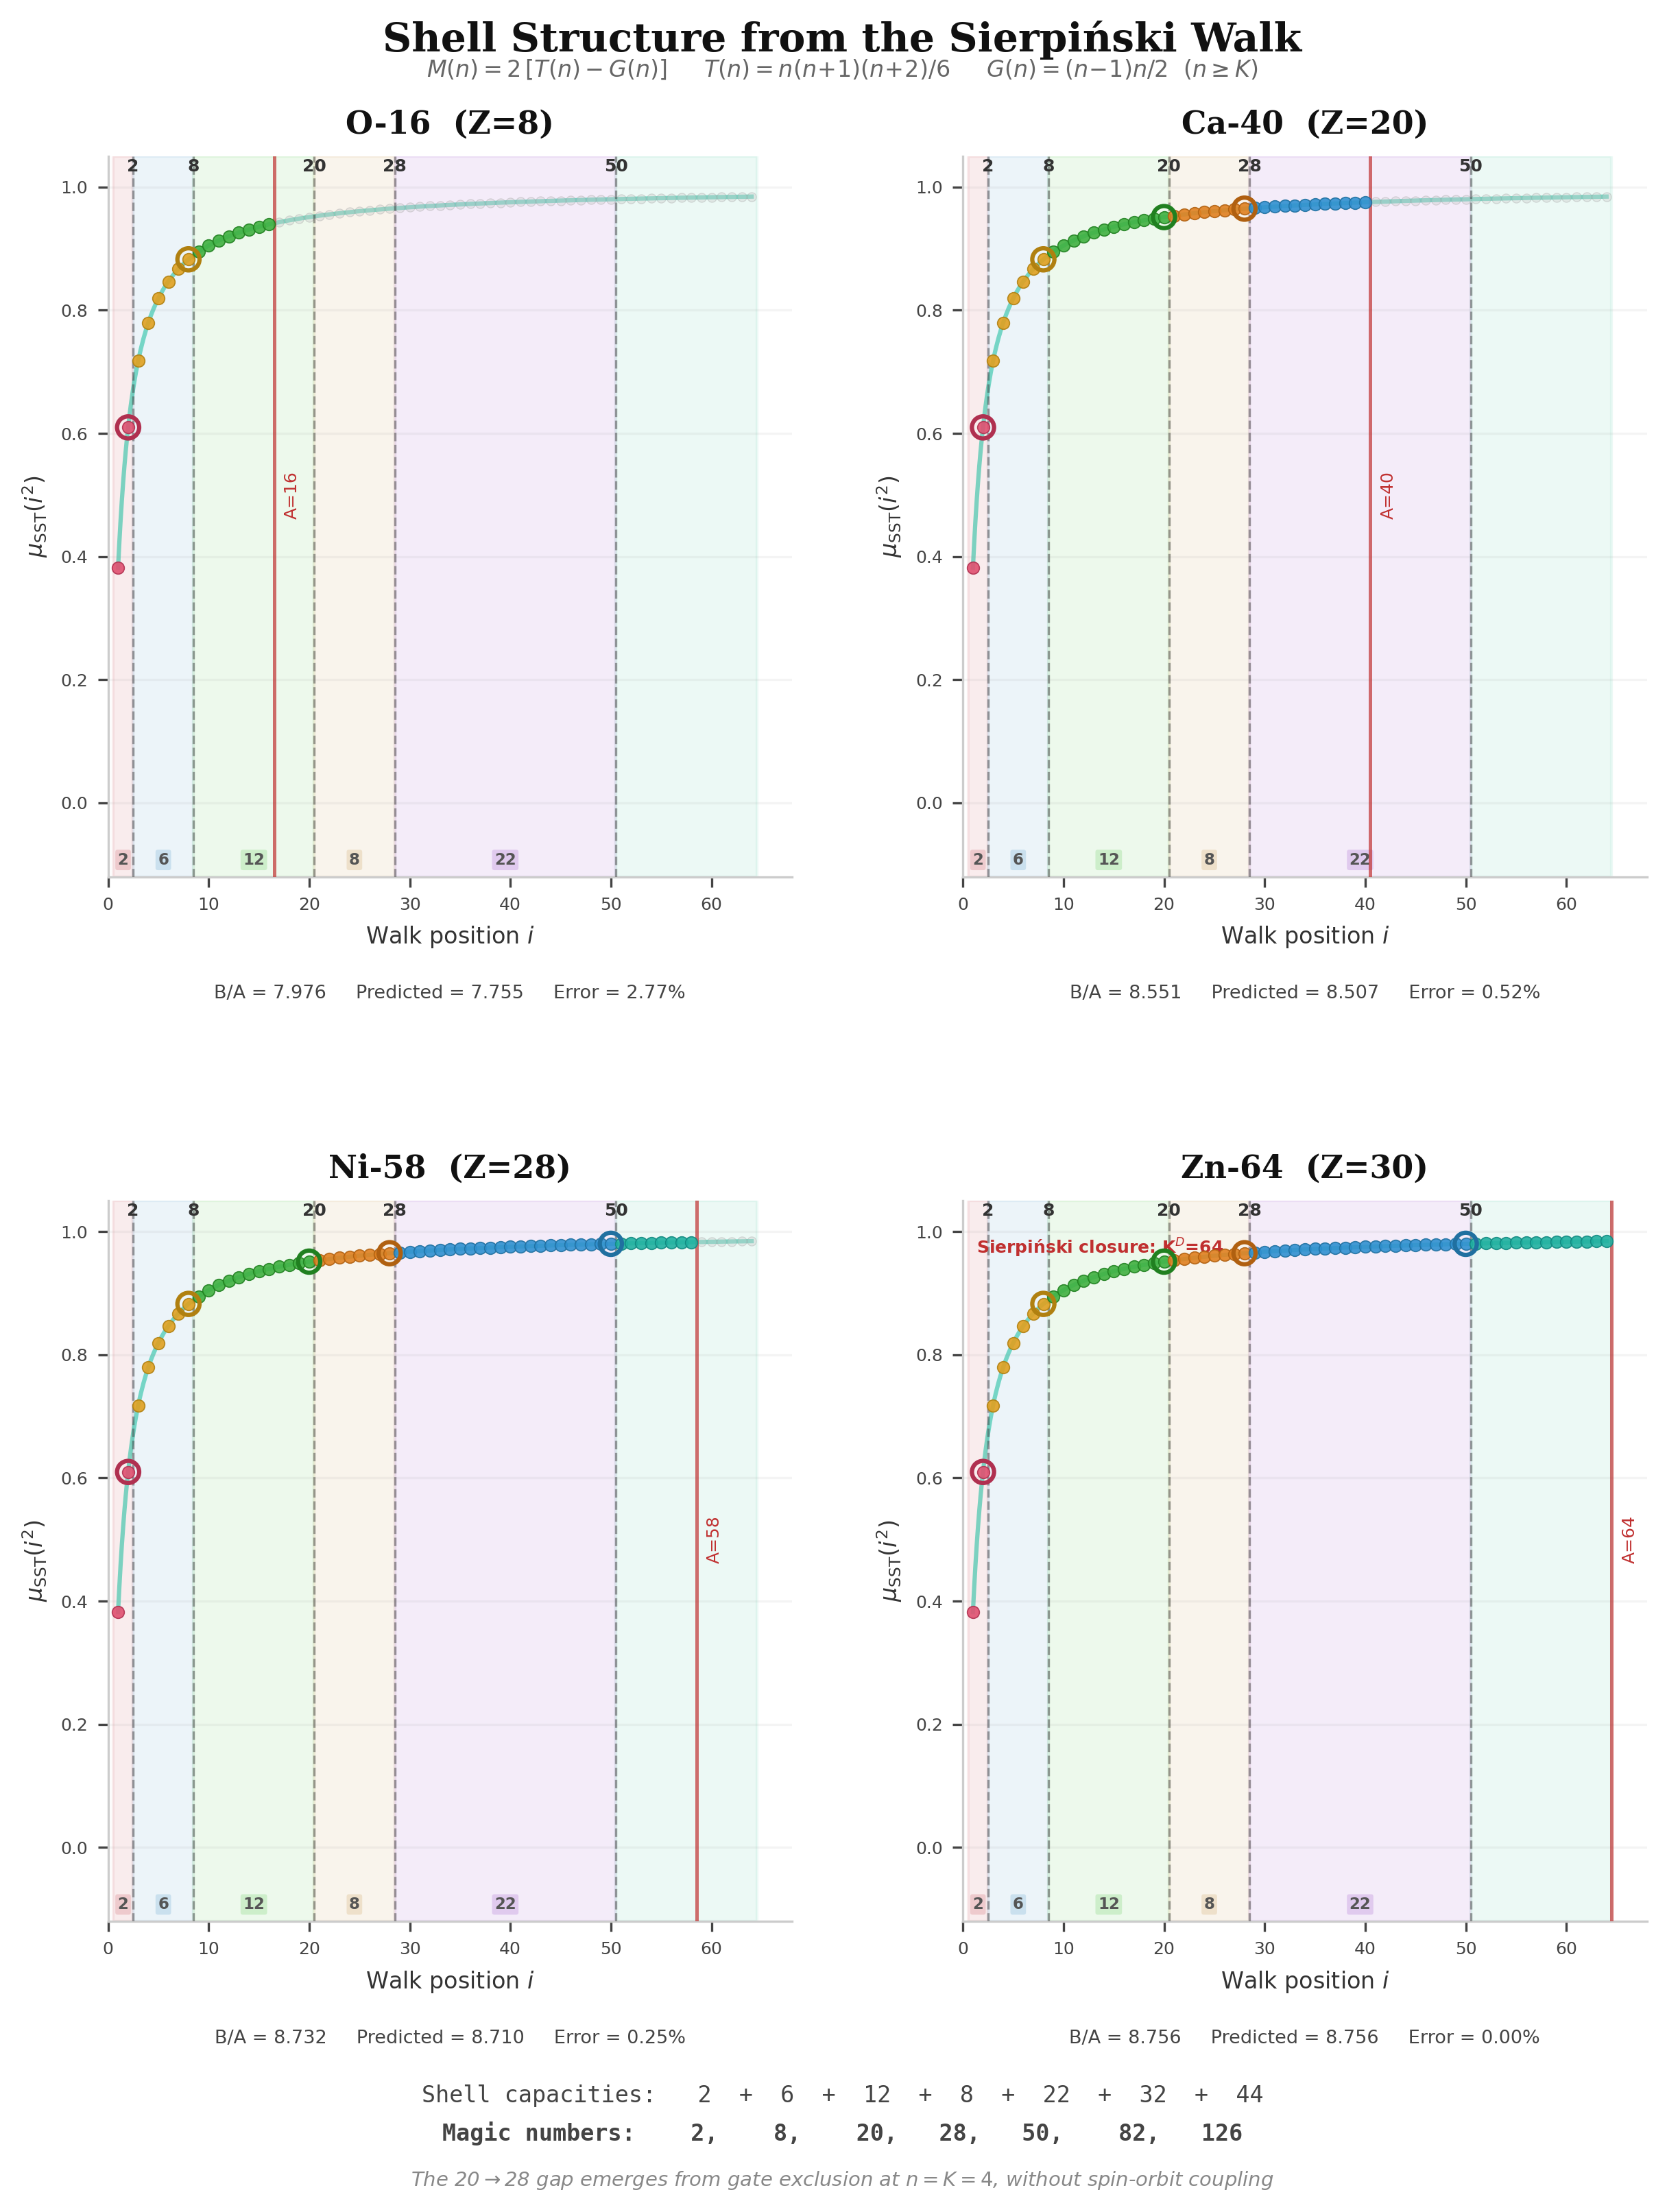
\includegraphics[width=0.95\textwidth]{gfd_shell_decomposition_4}
\caption{\textbf{Shell structure from the Sierpi\'nski walk.} The SST quadratic $\mu_{\mathrm{SST}}(i^2)$ at each walk position $i$, for four elements: O-16, Ca-40, Ni-58, and Zn-64. Coloured dots indicate occupied positions; grey dots are unfilled. Dashed vertical lines mark magic-number shell closures. Pastel bands show shell regions with capacities labelled at bottom. The narrow orange band (nucleon positions 21--28, capacity 8) is the gate-exclusion shell that reproduces the $20\!\to\!28$ gap without spin-orbit coupling.}
\label{fig:shells}
\end{figure*}

\subsection{Binding energy per nucleon}
\label{sec:binding}

The same $\mu_{\mathrm{SST}}$ that partitions the shells also gives the quantitative binding energy. For a nucleus with mass number $A$, define the coupling sum $\Sigma_A = \sum_{i=1}^{A}\mu_{\mathrm{SST}}(i^2)$. At $A = K^D = 64$, the walk is full and the sum completes one full sector: $\Sigma_{64} = 59.928$. The binding energy per nucleon is
\begin{equation}
\frac{B}{A}(A) = \frac{B}{A}(\mathrm{Zn})\;\frac{K^D}{A}\;\frac{\Sigma_A}{\Sigma_{K^D}}.
\label{eq:BA}
\end{equation}
Three terms set the result. $B/A(\mathrm{Zn}) = 8.756$\,MeV is the energy scale, calibrated from a single element: zinc-64, which sits at $A = K^D = 64$, the unique point where the walk fills completely. $K^D/A$ is the sharing factor: 64 positions of coupling shared among $A$ nucleons. $\Sigma_A/\Sigma_{64}$ is the coupling fraction: what share of the walk's total coupling has been collected. At $A = 64$ both ratios equal unity and Eq.~\ref{eq:BA} returns $B/A(\mathrm{Zn})$ by construction. A single element determines the energy scale; no further fitting is performed.

Eq.~\ref{eq:BA} describes the rising phase of the binding curve, which we label $\mathrm{SST}_1$. Each added nucleon contributes coupling, and $B/A$ increases. However, the experimental binding curve peaks near $A = 56$ and declines for heavier elements. The full curve requires understanding what happens when the walk fills and the structure continues onto its next sector.

\subsubsection{Sector crossings within the Sierpi\'nski hierarchy}
\label{sec:faces}

The Sierpi\'nski hierarchy has $K = 4$ sectors at its parent level, each containing $K^D = 64$ positions. The first 64 nucleons fill sector~0. At $A = 64$ that sector is complete. Additional nucleons continue onto the next sector, but crossing a sector boundary inverts the coupling profile: the SST reflects, and the binding energy descends from a ceiling value. Each sector transition produces a new descending curve because the field has already spent energy filling the previous sector.

Every descending curve has the same shape as $\mathrm{SST}_1$, subtracted from a ceiling:
\begin{equation}
\mathrm{SST}_{n}^{\,\mathrm{inv}}(A) = \mathrm{CEIL}_n - \mathrm{SST}_{\mathrm{local}}(A - A_n)
\end{equation}
where $\mathrm{SST}_{\mathrm{local}}$ evaluates the walk from position~1 to $(A - A_n)$ using Eq.~\ref{eq:BA}, and $A_n$ is the mass number where sector $n$ begins. The ceiling values are derived below.

\emph{Sector~0} ($A \leq 64$). $\mathrm{SST}_1$ rises from zero toward $8.756$\,MeV as the walk fills. Its inverse, $\mathrm{SST}_1^{\,\mathrm{inv}} = \mathrm{CEIL}_1 - \mathrm{SST}_1$, descends from $\mathrm{CEIL}_1$. For $A > 64$, $\mathrm{SST}_1^{\,\mathrm{inv}} < \mathrm{SST}_1$ and the descending curve governs. The binding energy turns over.

\emph{Sector~1} ($A > 64$). A new walk begins at $A = 64$, restarting from position~1. At $A = 100$, this walk has filled 36 of its 64 positions. At $A = 128$ it has filled all 64, completing a second sector. Its inverse, $\mathrm{SST}_2^{\,\mathrm{inv}} = \mathrm{CEIL}_2 - \mathrm{SST}_{\mathrm{local}}(A - 64)$, crosses below $\mathrm{SST}_1^{\,\mathrm{inv}}$ near $A \approx 110$ and governs the descent from tin toward lead.

\emph{Sector~2} ($A > 128$). A third walk begins at $A = 128$. Its inverse, $\mathrm{SST}_3^{\,\mathrm{inv}} = \mathrm{CEIL}_3 - \mathrm{SST}_{\mathrm{local}}(A - 128)$, governs the descent through the heavy elements.

\paragraph{Ceiling sequence.}
Each sector's inverse begins at a sector boundary and descends from a ceiling value. Every ceiling is set by one formula:
\begin{equation}
\mathrm{CEIL} = \frac{B}{A}(\mathrm{Zn}) + \frac{B}{A}\big|_{\mathrm{boundary}} - \mu_{\mathrm{SST}}(2)\,\bigg[\frac{B}{A}(\mathrm{Zn}) - \frac{B}{A}\big|_{\mathrm{boundary}}\bigg]
\label{eq:ceil}
\end{equation}
where $B/A|_{\mathrm{boundary}}$ is the predicted binding energy at the sector boundary from all previously established sectors, and
\begin{equation}
\mu_{\mathrm{SST}}(2) = \frac{(2 \cdot 2 + 1) - \sqrt{4 \cdot 2 + 1}}{2 \cdot 2} = \frac{5 - 3}{4} = \frac{1}{2}
\end{equation}
is the constitutive law at the bound-state field origin, the point where the coupling splits remaining capacity equally between forward and return directions.

Eq.~\ref{eq:ceil} is applied identically at each sector boundary:

\emph{Sector~0.} $B/A|_{\mathrm{boundary}} = B/A(\mathrm{Zn}) = 8.756$\,MeV (the walk has just filled; no prior sector). The $\mu_{\mathrm{SST}}(2)$ correction is $\tfrac{1}{2}[8.756 - 8.756] = 0$. No impedance. $\mathrm{CEIL}_1 = 8.756 + 8.756 - 0 = 17.512$\,MeV.

\emph{Sector~1.} $B/A|_{\mathrm{boundary}} = \mathrm{SST}_1^{\,\mathrm{inv}}(128) = 17.512 - 9.003 = 8.509$\,MeV (the field value at $A = 128$ from sector~0). The $\mu_{\mathrm{SST}}(2)$ correction is $\tfrac{1}{2}[8.756 - 8.509] = 0.124$\,MeV. $\mathrm{CEIL}_2 = 8.756 + 8.509 - 0.124 = 17.141$\,MeV.

\emph{Sector~2.} $B/A|_{\mathrm{boundary}} = \mathrm{CEIL}_2 - B/A(\mathrm{Zn}) = 17.141 - 8.756 = 8.385$\,MeV (the field value at $A = 128$ updated by sector~1). The $\mu_{\mathrm{SST}}(2)$ correction is $\tfrac{1}{2}[8.756 - 8.385] = 0.186$\,MeV. $\mathrm{CEIL}_3 = 8.756 + 8.385 - 0.186 = 16.955$\,MeV.

\begin{table}
\centering
\caption{Ceiling sequence from Eq.~\ref{eq:ceil}. One formula, one factor $\mu_{\mathrm{SST}}(2) = \tfrac{1}{2}$, three applications.}
\label{tab:ceilings}
\begin{tabular}{cccc}
\hline
Sector & $B/A|_{\mathrm{boundary}}$ (MeV) & Correction (MeV) & Ceiling (MeV) \\
\hline
0 & 8.756 & 0.000 (no impedance) & 17.512 \\
1 & 8.509 & 0.124 & 17.141 \\
2 & 8.385 & 0.186 & 16.955 \\
\hline
\end{tabular}
\end{table}

The same constitutive law that shapes the binding curve also governs the ceiling at every sector boundary.

At every mass number, the predicted binding energy is the minimum of all active curves:
\begin{equation}
\frac{B}{A} = \min\!\big(\mathrm{SST}_1,\;\mathrm{SST}_1^{\,\mathrm{inv}},\;\mathrm{SST}_2^{\,\mathrm{inv}},\;\mathrm{SST}_3^{\,\mathrm{inv}}\big).
\label{eq:envelope}
\end{equation}

As Fig.~\ref{fig:binding} shows, the envelope tracks the experimental curve across the full range. The fit is tighter in the post-64 region ($R^2 = 0.96$, MAE $= 36$\,keV) than in the first sector ($R^2 = 0.90$, MAE $= 97$\,keV); across the full range from helium to lead, $R^2 = 0.82$ and MAE $= 95$\,keV. Te-128, which sits at $A = 2K^D = 128$, is predicted to within 14\,keV.

\begin{figure*}
\centering
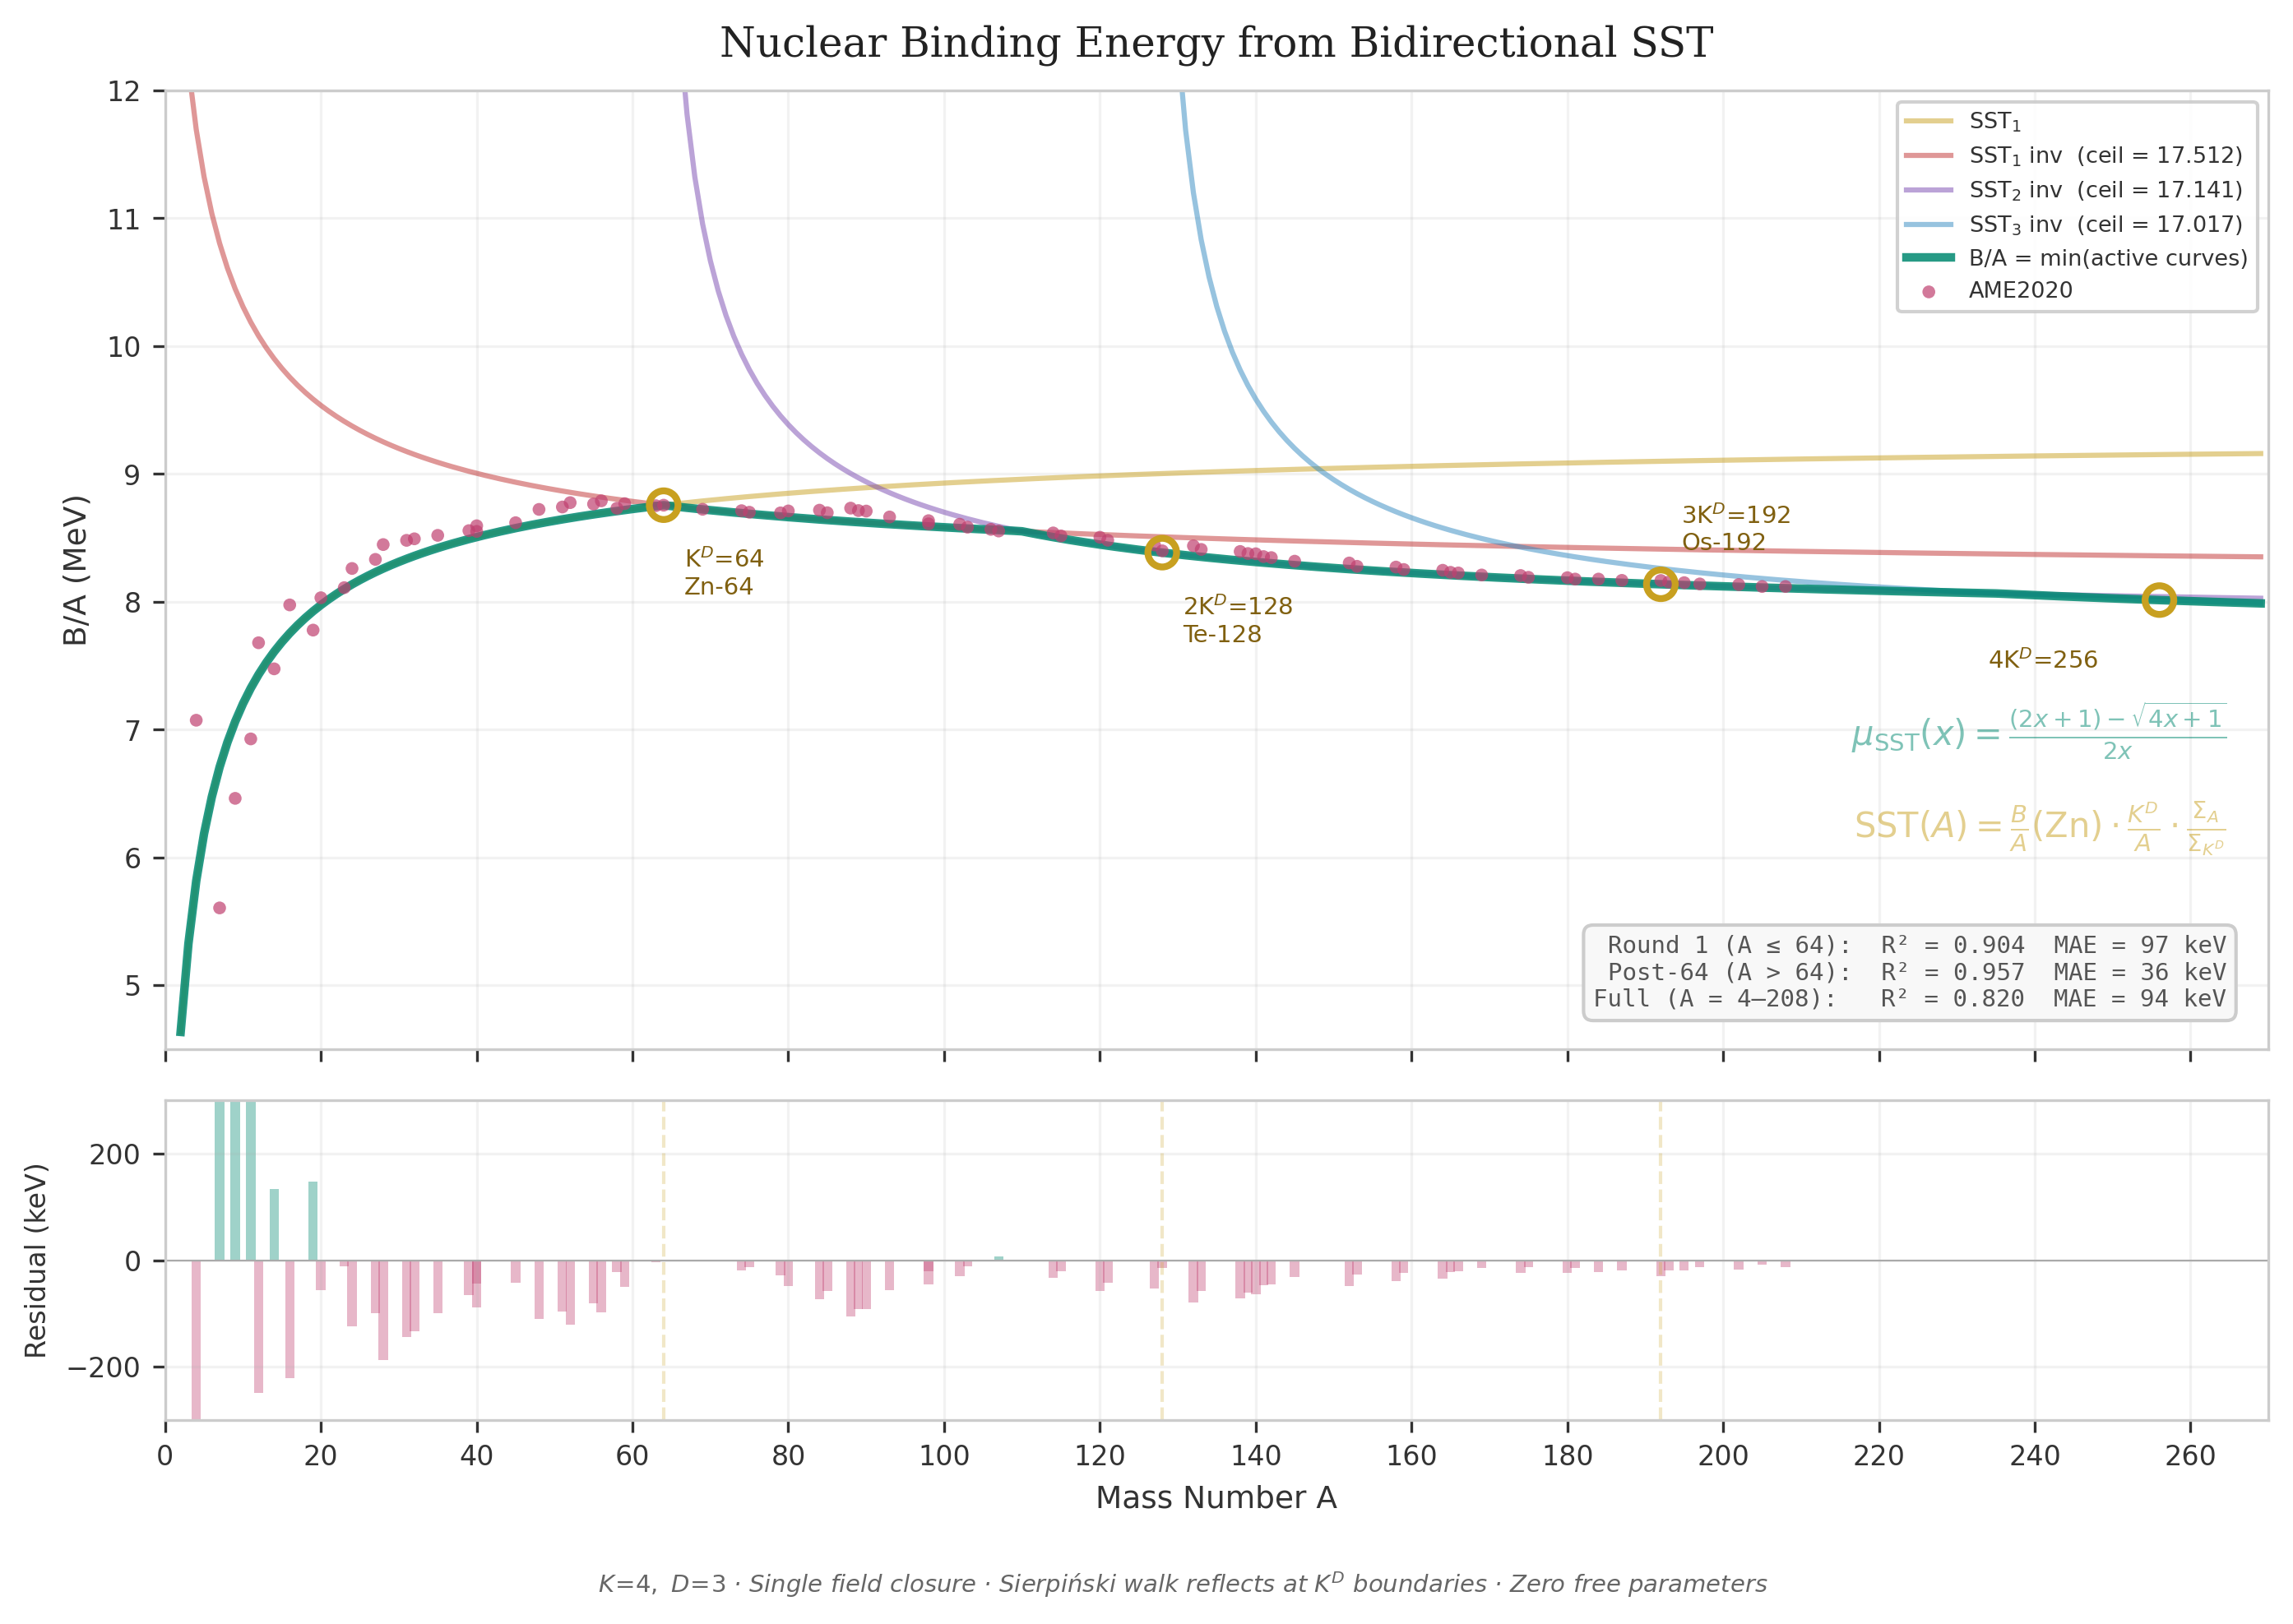
\includegraphics[width=0.95\textwidth]{gfd_binding_energy}
\caption{\textbf{Binding energy per nucleon from the SST quadratic.} Gold: $\mathrm{SST}_1$ (rising curve, walk filling). Red: $\mathrm{SST}_1^{\,\mathrm{inv}}$ (sector~0 reflection, ceiling at $17.512$\,MeV). Purple: $\mathrm{SST}_2^{\,\mathrm{inv}}$ (sector~1 reflection, ceiling at $17.141$\,MeV). Blue: $\mathrm{SST}_3^{\,\mathrm{inv}}$ (sector~2 reflection, ceiling at $16.955$\,MeV). Teal: $B/A = \min(\text{active curves})$, the model prediction. Pink dots: AME2020 experimental data. Yellow circles mark the Sierpi\'nski sector-fill boundaries at $K^D = 64$ (Zn), $2K^D = 128$ (Te), and $3K^D = 192$ (Os). Residuals are shown in the lower panel.}
\label{fig:binding}
\end{figure*}

\subsection{The Sierpi\'nski walk}
\label{sec:sierpinski}

The binding curve and the shell structure share a common origin: the 64-position Sierpi\'nski walk (Sec.~\ref{sec:walk}). As Fig.~\ref{fig:sierpinski} shows, the progressive filling of the walk tracks both the shell closures and the rising $B/A$.

A central feature of the structure is that binding energy is distributed \emph{equally} across all occupied positions: every occupied tile receives the same $B/A$. The $\mu_{\mathrm{SST}}(i^2)$ values at each position are not individual nucleon energies; they are each position's coupling contribution to building the collective total. The structure sums these contributions and shares the result uniformly.

This is why the binding energy per nucleon is a ratio: total binding divided by $A$, so that each nucleon receives the average. The curve rises because adding nucleons adds coupling (each new $\mu_{\mathrm{SST}}$ term is positive and near unity for large $i$). The curve saturates because $\mu_{\mathrm{SST}} \to 1$ for large $x$: additional positions contribute less and less marginal coupling.

At $A = 64$ sector~0 is full. The walk continues onto the next sector of the Sierpi\'nski hierarchy (Sec.~\ref{sec:faces}), and the coupling profile inverts. Visually, the triangle remains fully lit, but the number inside each tile decreases: $8.76$\,MeV for Zn-64 (sector~0 full), $8.45$\,MeV for Sn-120 (sector~1 partially filled), $8.11$\,MeV for Pb-208. The declining $B/A$ past iron is the cost of crossing sector boundaries within the same 64-position structure.

The eight elements shown range from C-12 (12 of 64 positions filled) to Zn-64 (all 64 filled), with the error shrinking from 249\,keV at carbon to 0\,keV at zinc.

\begin{figure*}
\centering
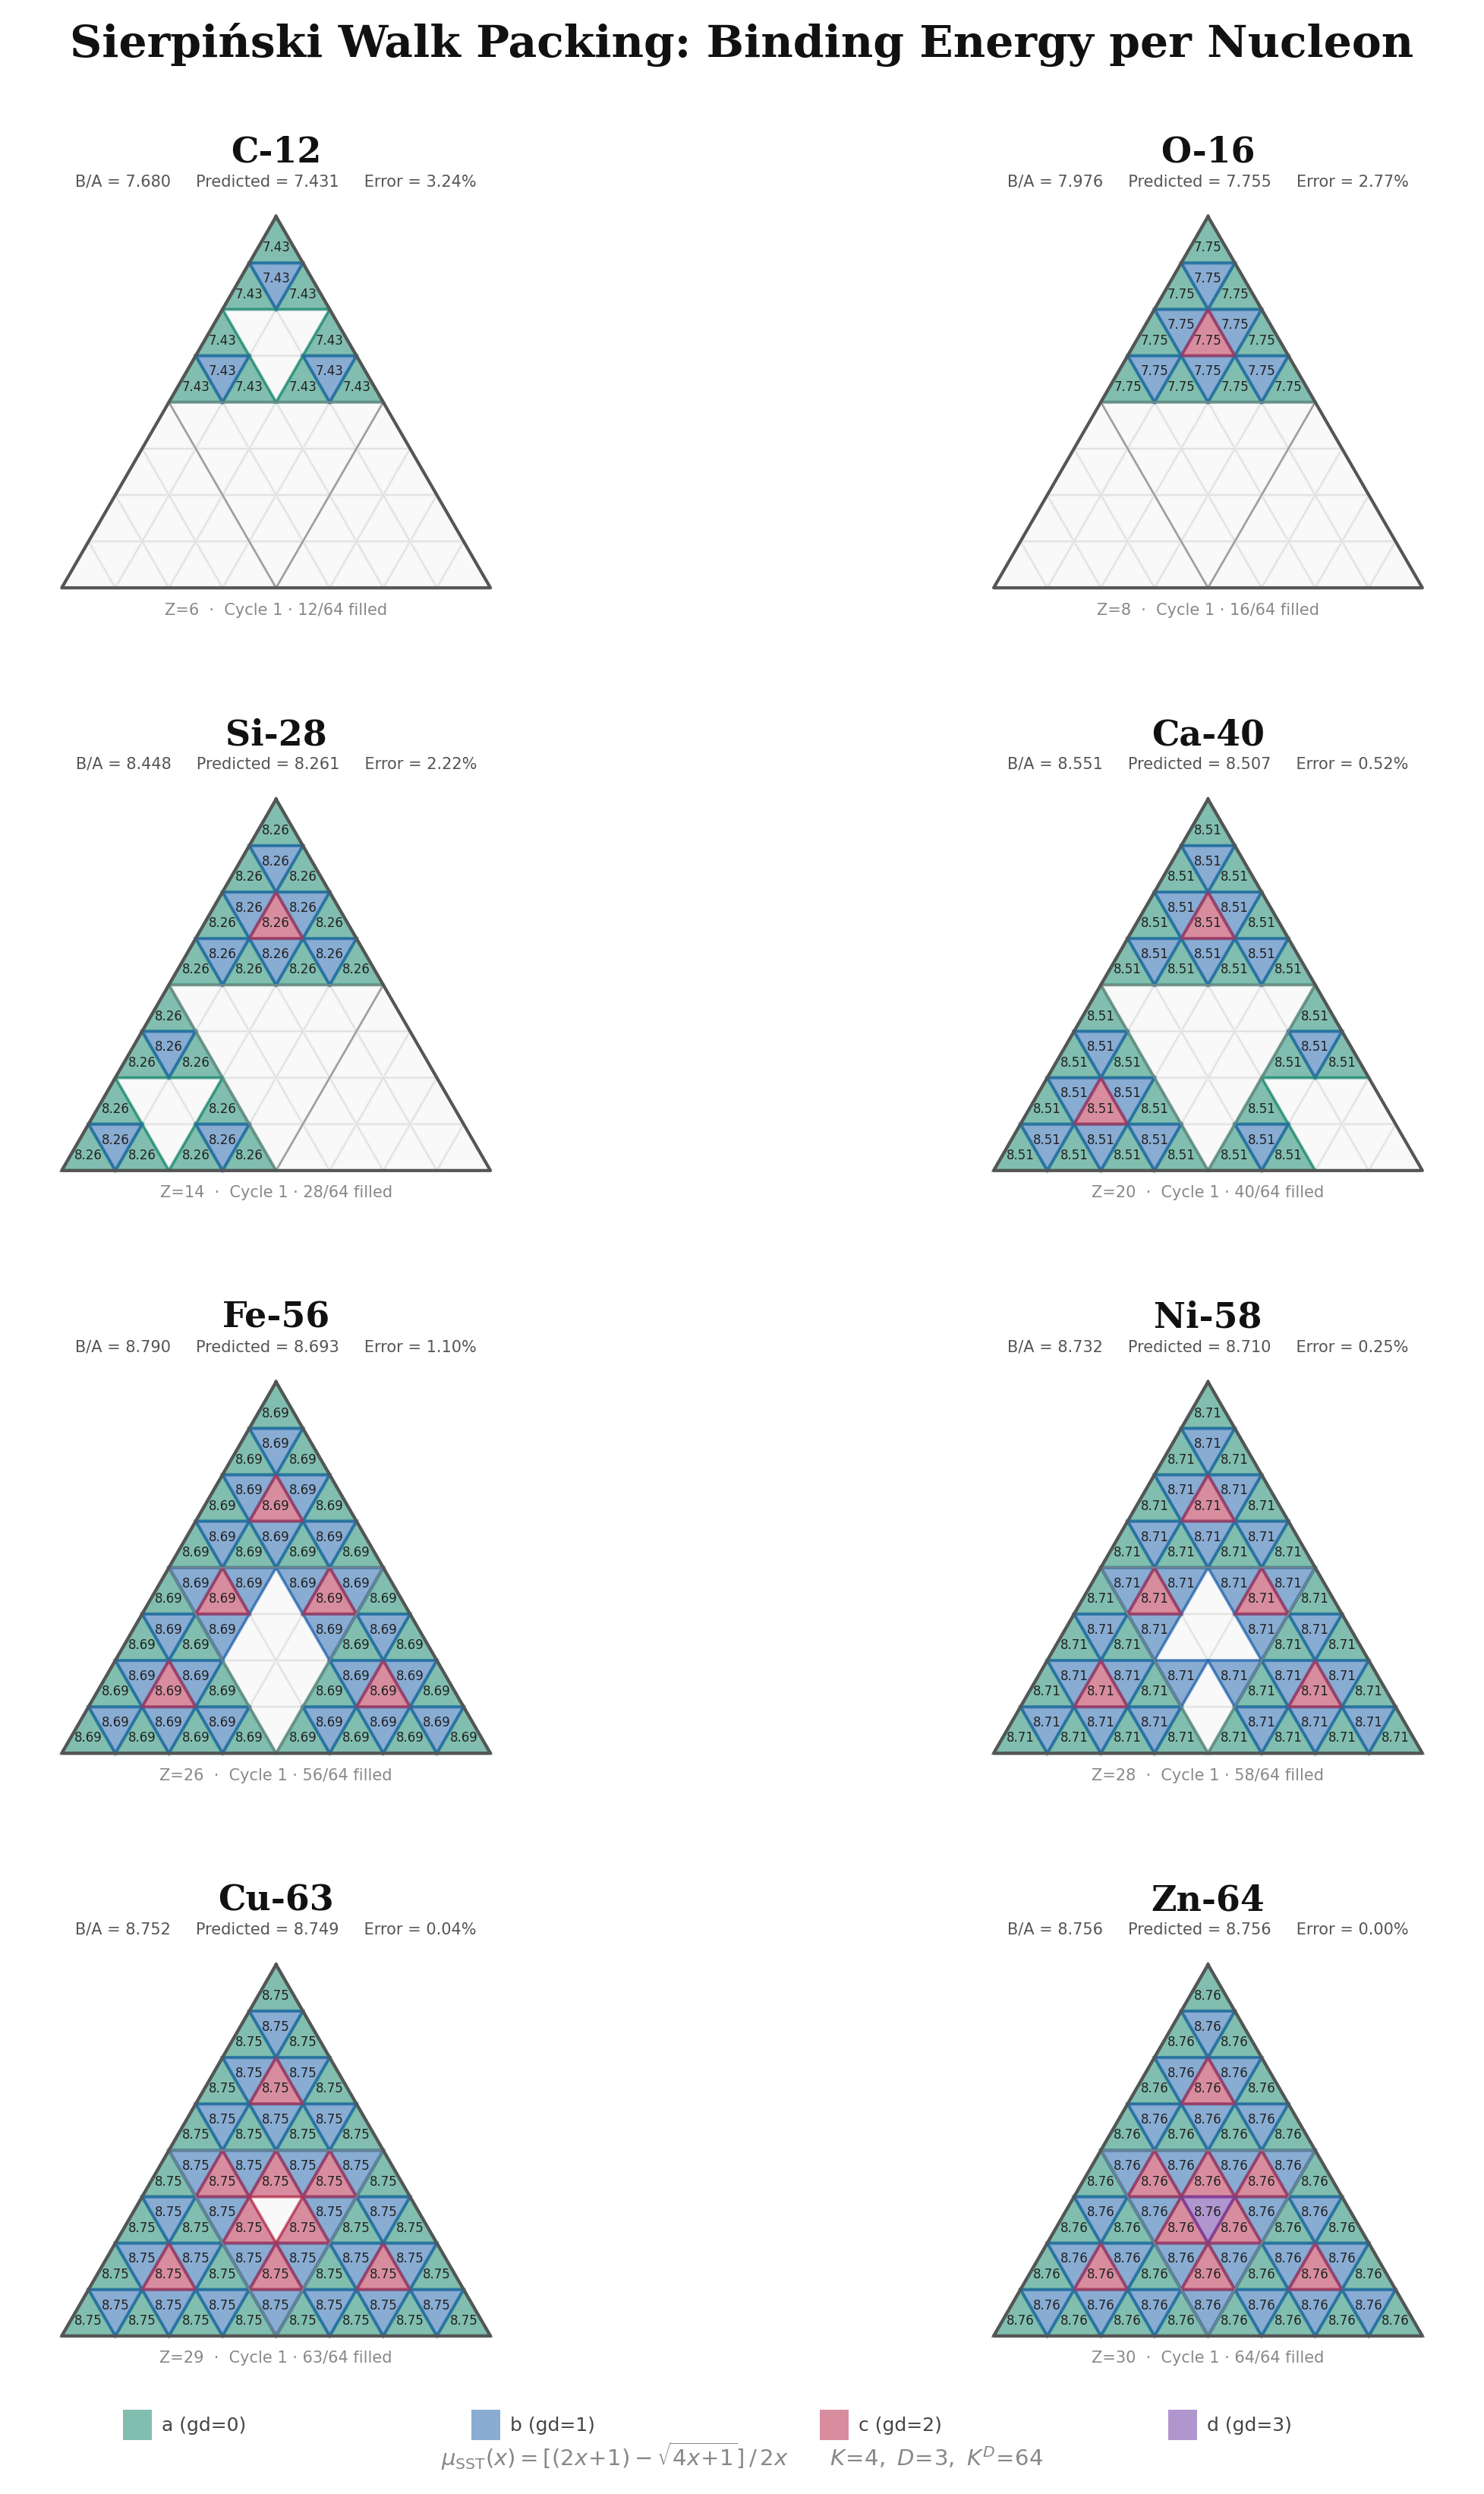
\includegraphics[width=0.95\textwidth]{gfd_sierpinski_packing_8}
\caption{\textbf{Sierpi\'nski walk packing.} Eight elements from C-12 to Zn-64, showing the 64-position walk filling progressively. Each filled tile displays the predicted $B/A$ for that element (all tiles show the same value; binding is distributed equally). Colours indicate gate depth within the fractal structure. The error decreases from 249\,keV (C-12) to 0\,keV (Zn-64, full closure at $K^D = 64$).}
\label{fig:sierpinski}
\end{figure*}

% ----------------------------------------------------------------------------
% 4. DISCUSSION
% ----------------------------------------------------------------------------
\section{Discussion}
\label{sec:discussion}

The SST quadratic produces three outputs from one equation: algebraically exact magic numbers, a quantitative binding curve, and the Sierpi\'nski walk that connects them. We turn now to scope, limitations, and the cross-scale connection.

\subsection{What is new}

The Bethe-Weizs\"acker formula fits the binding curve with five parameters; the nuclear shell model predicts magic numbers with a phenomenological spin-orbit term. Each addresses one side of the problem. The SST quadratic addresses both from a single equation with zero free parameters: the magic numbers come from the packing algebra (Eq.~\ref{eq:magic}), which uses only $K = 4$ and the gate threshold, and the binding curve comes from the same $\mu_{\mathrm{SST}}$ evaluated along the walk (Eq.~\ref{eq:BA}), calibrated from a single element. The $20\!\to\!28$ gap is structural: the gate face activates at $n = K$, excluding positions, with no spin-orbit term introduced.

\subsection{Cross-scale connection}

The SST that decodes galaxy rotation curves (Sec.~\ref{sec:sst}) takes two forms depending on whether the coupling is one-directional or self-consistent. The galactic constitutive law is $\mu(x) = x/(1+x)$, the one-directional solution of the SST. The nuclear constitutive law is $\mu_{\mathrm{SST}}(x)$ from Eq.~\ref{eq:musst}, the self-consistent solution when the SST closes on itself in a bound state.

Both emerge from the same field equation: the one-directional solution governs unbound systems (galaxies, where matter sources the field), and the self-consistent solution governs bound systems (nuclei, where the field sources itself). The structural constants $K = 4$ and $D = 3$ are the same in both cases. The transition between regimes is the SST itself.

\subsection{Limitations}

Light elements ($A < 12$) show residuals of 200\,keV or more. These are few-body systems where the continuous approximation of the sum in Eq.~\ref{eq:BA} is at its weakest. The Sierpi\'nski walk is a bulk structure, and nuclei with only a handful of occupied positions do not yet benefit from the statistical averaging that improves accuracy at larger $A$.

The sector-crossing construction reproduces the shape of the binding curve from helium to lead, but the detailed oscillations at shell closures (the fine structure of the curve) require the next layer of the framework: the shell-by-shell decomposition of $\mu_{\mathrm{SST}}$ contributions. This is deferred to a longer treatment.

\subsection{Stability at lead}

The Sierpi\'nski hierarchy has $K = 4$ sectors. Sectors 0, 1, and 2 are ordinary sectors, each holding $K^D = 64$ positions, for a total of $3 \times K^D = 192$. The fourth sector (index~3) is the gate sector, the structural boundary of the Sierpi\'nski hierarchy where the walk closes on itself. Experimentally, stability persists through Pb-208 ($A = 208$) but not beyond; Pb-208 is the heaviest stable nucleus and the endpoint of every alpha decay chain. The 16 positions beyond $A = 192$ fall within the gate sector, at the boundary where the hierarchy closes. Beyond this point, nuclei decay.

% ----------------------------------------------------------------------------
% 5. CONCLUSIONS
% ----------------------------------------------------------------------------
\section{Conclusions}
\label{sec:conclusions}

The bound-state partition of the scalar-tensor transition, the SST quadratic $\mu_{\mathrm{SST}}(x) = [(2x+1) - \sqrt{4x+1}]/2x$, produces three independently verifiable results:

\begin{enumerate}
\item \textbf{Magic numbers.} $M(n) = 2[T(n) - G(n)]$ gives 2, 8, 20, 28, 50, 82, 126. The $20\!\to\!28$ gap emerges from gate exclusion at $n = K = 4$, without spin-orbit coupling.
\item \textbf{Binding energy.} $B/A = B/A(\mathrm{Zn})\,(K^D/A)\,(\Sigma_A/\Sigma_{K^D})$, reflected at each sector boundary of the Sierpi\'nski hierarchy, reproduces the binding curve from He to Pb at MAE $= 95$\,keV. One calibration point (Zn-64).
\item \textbf{Cross-scale unity.} The same SST that decodes galaxy rotation curves predicts nuclear binding when applied self-consistently. One field equation, two domains, zero free parameters in both.
\end{enumerate}

The magic numbers follow from elementary arithmetic on the packing formula, and the binding curve from evaluating the SST quadratic along the walk. The figures and equations in this letter are self-contained; the supplementary material provides scripts for full numerical reproduction.

\section{Data and Code Availability}
\label{sec:data}
Experimental binding energies are from the Atomic Mass Evaluation 2020 \citep{AME2020}. Python scripts for all three figures and the 30-test validation harness are available at \texttt{github.com/field-dynamics/nuclear-binding} and at \texttt{docs.fielddynamics.org}. Supplementary material: validation test suite, element-by-element predictions, and derivation of the SST quadratic from the self-consistency condition.

% ----------------------------------------------------------------------------
% REFERENCES
% ----------------------------------------------------------------------------
\bibliographystyle{mnras}

\begin{thebibliography}{99}
\bibitem[\protect\citeauthoryear{Bethe \& Weizs\"acker}{1935}]{BW1935}
Bethe H.~A., 1936, Rev.\ Mod.\ Phys., 8, 82; Weizs\"acker C.~F.~von, 1935, Z.\ Phys., 96, 431

\bibitem[\protect\citeauthoryear{Mayer}{1949}]{Mayer1949}
Mayer M.~G., 1949, Phys.\ Rev., 75, 1969

\bibitem[\protect\citeauthoryear{Wang et al.}{2021}]{AME2020}
Wang M., Huang W.~J., Kondev F.~G., Audi G., Naimi S., 2021, Chinese Phys.\ C, 45, 030003

\bibitem[\protect\citeauthoryear{Nelson}{2026}]{Nelson2026}
Nelson S., 2026, MNRAS (submitted), ``Gravity Field Dynamics: Decoding mass from observed rotation curves''
\end{thebibliography}

\end{document}
